% ============================================================================
% EST-744 — Clase 4: Mecanismos de Atención
% Diagramas TikZ — archivo consolidado
%
% Contiene 10 diagramas standalone, compilables de dos maneras:
%
%   A) Documento completo (todos los diagramas en páginas separadas):
%      pdflatex clase_4_diagramas_tikz.tex
%
%   B) Diagrama individual (copiar el bloque tikzpicture al preámbulo propio):
%      \documentclass[border=8pt]{standalone}
%      \usepackage{tikz}
%      \usetikzlibrary{arrows.meta,positioning,fit,backgrounds}
%      \begin{document}
%        ... pegar bloque tikzpicture ...
%      \end{document}
%
% NOTA: No usar \usepackage[T1]{fontenc} — genera errores de fuente EC
%       en algunas distribuciones TeX Live. Los diagramas usan \sffamily
%       directamente.
%
% Esquema de colores (consistente con Clase 1 y Clase 3):
%   blue!12–20   → entradas / embeddings
%   orange!18–30 → capas internas / celdas recurrentes
%   green!18–45  → salidas / pesos altos
%   gray!8–22    → capas auxiliares (norm, pooling)
%   red!8–10     → advertencias / problemas
% ============================================================================

\documentclass[12pt, a4paper]{article}
\usepackage{tikz}
\usetikzlibrary{arrows.meta, positioning, fit, backgrounds}
\usepackage{caption}
\usepackage{geometry}
\geometry{margin=2cm}
\pagestyle{empty}

\begin{document}

% ----------------------------------------------------------------------------
% DIAGRAMA 1: Cuello de botella RNN secuencial
% Lámina: "El Problema: Cuello de Botella Secuencial"
% ----------------------------------------------------------------------------
\begin{figure}[h]\centering
\begin{tikzpicture}[
  font=\sffamily\small,
  cell/.style={draw, rounded corners=3pt, thick,
               fill=orange!20, minimum width=1.3cm, minimum height=1.1cm},
  word/.style={draw, circle, thick, fill=blue!15,
               minimum size=0.9cm, inner sep=1pt, font=\sffamily\footnotesize},
  arr/.style={-{Stealth[length=2.2mm]}, thick},
  seq/.style={-{Stealth[length=2.2mm]}, thick, orange!70!black, dashed}
]
\node[word] (w0) at (0,0)    {\textit{La}};
\node[word] (w1) at (2.2,0)  {\textit{película}};
\node[word] (w2) at (4.4,0)  {\textit{fue}};
\node[word] (w3) at (6.6,0)  {\textit{genial}};
\node[cell] (r0) at (0,2)    {$h_1$};
\node[cell] (r1) at (2.2,2)  {$h_2$};
\node[cell] (r2) at (4.4,2)  {$h_3$};
\node[cell] (r3) at (6.6,2)  {$h_4$};
\node[font=\sffamily\scriptsize, text=gray] at (0,  3.0) {$t=0$};
\node[font=\sffamily\scriptsize, text=gray] at (2.2,3.0) {$t=1$};
\node[font=\sffamily\scriptsize, text=gray] at (4.4,3.0) {$t=2$};
\node[font=\sffamily\scriptsize, text=gray] at (6.6,3.0) {$t=100$};
\draw[arr] (w0)--(r0); \draw[arr] (w1)--(r1);
\draw[arr] (w2)--(r2); \draw[arr] (w3)--(r3);
\draw[seq] (r0) -- node[above,font=\sffamily\scriptsize]{espera} (r1);
\draw[seq] (r1) -- node[above,font=\sffamily\scriptsize]{espera} (r2);
\node at (5.5,2) {\large$\cdots$};
\draw[seq] (r2)--(5.1,2); \draw[seq] (5.9,2)--(r3);
\node[align=left, font=\sffamily\scriptsize, text=red!70!black, text width=3cm]
  at (9.4,2) {¡Debe recordar\\todo desde\\100 pasos atrás!};
\draw[-{Stealth[length=1.8mm]}, red!60!black, thick] (8.3,2)--(r3.east);
\node[draw, rounded corners, fill=red!8, font=\sffamily\small,
      text=red!70!black, inner sep=4pt]
  at (3.3,-1.1) {Procesamiento \textbf{secuencial}: cada paso bloquea al siguiente};
\end{tikzpicture}
\caption*{D1 — Cuello de botella RNN}
\end{figure}

\newpage

% ----------------------------------------------------------------------------
% DIAGRAMA 2: Selección suave / foco de atención por relevancia
% Lámina: "Selección Suave"
% ----------------------------------------------------------------------------
\begin{figure}[h]\centering
\begin{tikzpicture}[
  font=\sffamily\small,
  word/.style={draw, rounded corners=3pt, thick,
               minimum width=2.0cm, minimum height=0.75cm,
               inner sep=3pt, align=center},
  arr/.style={-{Stealth[length=2.5mm]}, thick},
  lbl/.style={font=\sffamily\scriptsize, align=left}
]
\node[draw, rounded corners=4pt, fill=blue!15, thick,
      minimum width=2.4cm, minimum height=0.8cm, font=\sffamily\small]
  (q) at (0,0) {\textit{genial}};
\node[font=\sffamily\scriptsize, text=blue!60!black, above=0.08cm of q]
  {Consulta ($Q$): ¿qué busco?};
\node[word, fill=red!15,   minimum width=1.0cm] (p0) at (4.5, 2.1) {\textit{La}};
\node[lbl, right=0.2cm of p0, text=gray] {$0.05$ — relleno};
\draw[arr, gray] (q.east) to[out=10,in=180] (p0.west);
\node[word, fill=orange!25, minimum width=1.8cm] (p1) at (4.5, 0.7) {\textit{película}};
\node[lbl, right=0.2cm of p1] {$0.15$ — contexto};
\draw[arr, orange!70!black] (q.east) to[out=5,in=180] (p1.west);
\node[word, fill=orange!40, minimum width=2.1cm] (p2) at (4.5,-0.7) {\textit{fue}};
\node[lbl, right=0.2cm of p2] {$0.20$ — modificador};
\draw[arr, orange!80!black, thick] (q.east) to[out=-5,in=180] (p2.west);
\node[word, fill=green!45,  minimum width=3.3cm, very thick] (p3) at (4.5,-2.1) {\textit{genial}};
\node[lbl, right=0.2cm of p3, text=green!50!black, font=\sffamily\scriptsize\bfseries]
  {$0.60$ — señal fuerte};
\draw[arr, green!50!black, line width=2pt] (q.east) to[out=-10,in=180] (p3.west);
\node[draw, rounded corners, fill=gray!8, inner sep=5pt,
      font=\sffamily\scriptsize, align=left, text width=3.6cm]
  at (0,-3.3) {Grosor de la flecha $\propto$ peso de atención};
\end{tikzpicture}
\caption*{D2 — Selección suave}
\end{figure}

\newpage

% ----------------------------------------------------------------------------
% DIAGRAMA 3: Ejemplo numérico QKV paso a paso
% Lámina: "Ejemplo Numérico de Atención"
% ----------------------------------------------------------------------------
\begin{figure}[h]\centering
\begin{tikzpicture}[
  font=\sffamily\small,
  word/.style={draw, rounded corners=3pt, thick, fill=blue!12,
               minimum width=1.55cm, minimum height=0.7cm, align=center},
  blk/.style={draw, rounded corners=3pt, thick, fill=gray!8,
               inner sep=6pt, align=left, text width=8.8cm},
  hl/.style={draw, rounded corners=3pt, thick, fill=green!25,
             minimum width=1.55cm, minimum height=0.7cm, align=center},
  arr/.style={-{Stealth[length=2mm]}, thick}
]
\node[font=\sffamily\small\bfseries, anchor=west] at (-0.2,4.8) {Oración:};
\node[word] (La)   at (1.8,4.8) {\textit{La}};
\node[word] (peli) at (3.4,4.8) {\textit{pelicula}};
\node[hl]   (fue)  at (5.0,4.8) {\textbf{\textit{fue}}};
\node[word] (gen)  at (6.6,4.8) {\textit{genial}};
\node[font=\sffamily\scriptsize, text=gray] at (1.8,4.1) {pos 0};
\node[font=\sffamily\scriptsize, text=gray] at (3.4,4.1) {pos 1};
\node[font=\sffamily\scriptsize, text=green!50!black, font=\sffamily\scriptsize\bfseries]
  at (5.0,4.1) {consulta};
\node[font=\sffamily\scriptsize, text=gray] at (6.6,4.1) {pos 3};
\node[blk] (p1) at (4.4,2.8) {
  \textbf{Paso 1} — Similitud (consulta ``fue'' vs.\ cada clave):\\[2pt]
  \hspace{6pt}``fue'' vs ``La'':\hfill $-0.20$\\
  \hspace{6pt}``fue'' vs ``pelicula'':\hfill $\phantom{-}0.30$\\
  \hspace{6pt}``fue'' vs ``fue'':\hfill $\phantom{-}1.00$
    \quad {\scriptsize$\leftarrow$ se reconoce a si misma}\\
  \hspace{6pt}``fue'' vs ``genial'':\hfill $\phantom{-}0.50$
};
\node[blk] (p2) at (4.4,1.15) {
  \textbf{Paso 2} — Softmax $\rightarrow$ pesos de atenci\'on:\\[2pt]
  \hspace{6pt}$[\,0.05,\quad 0.15,\quad 0.60,\quad 0.20\,]$\\
  \hspace{6pt}$\underbrace{\hspace{0.9cm}}_{La}\quad
               \underbrace{\hspace{1.1cm}}_{pelicula}\quad
               \underbrace{\hspace{0.9cm}}_{fue}\quad
               \underbrace{\hspace{1.1cm}}_{genial}$
};
\node[blk] (p3) at (4.4,-0.45) {
  \textbf{Paso 3} — Combinaci\'on ponderada de valores:\\[2pt]
  \hspace{6pt}salida $=\;0.05\,v_{La}
    + 0.15\,v_{pel} + 0.60\,v_{fue} + 0.20\,v_{genial}$
};
\draw[arr] (fue.south) -- ++(0,-0.45) -- (p1.north);
\end{tikzpicture}
\caption*{D3 — Ejemplo numérico QKV}
\end{figure}

\newpage

% ----------------------------------------------------------------------------
% DIAGRAMA 4: Atención multi-cabezal
% Lámina: "Atención Multi-Cabezal"
% ----------------------------------------------------------------------------
\begin{figure}[h]\centering
\begin{tikzpicture}[
  font=\sffamily\small,
  head/.style={draw, rounded corners=3pt, thick,
               minimum width=3.6cm, minimum height=0.75cm,
               inner sep=4pt, align=left},
  inp/.style={draw, rounded corners=3pt, fill=blue!12, thick,
              minimum width=5.4cm, minimum height=0.7cm, align=center},
  outbox/.style={draw, rounded corners=3pt, fill=green!18, thick,
                 minimum width=5.4cm, minimum height=0.7cm, align=center},
  proj/.style={draw, rounded corners=3pt, fill=gray!15, thick,
               minimum width=5.4cm, minimum height=0.7cm, align=center},
  arr/.style={-{Stealth[length=2.2mm]}, thick}
]
\node[inp] (x) at (0,5.5) {$x$ \small(embedding + posici\'on)};
\node[head, fill=orange!18] (h1) at (-3.5,3.8)
  {\textbf{Cabeza 1}\\\scriptsize similitud sem\'antica\\[-1pt]
   \scriptsize ``pel\'icula'' $\leftrightarrow$ ``film''};
\node[head, fill=orange!22] (h2) at (0,3.8)
  {\textbf{Cabeza 2}\\\scriptsize rol gramatical\\[-1pt]
   \scriptsize sujeto, objeto, verbo};
\node[head, fill=orange!26] (h3) at (3.5,3.8)
  {\textbf{Cabeza 3\,\ldots\,8}\\\scriptsize modificadores,\\[-1pt]
   \scriptsize largo alcance, \ldots};
\draw[arr] (x.south)--++(0,-0.25)-|(h1.north);
\draw[arr] (x.south)--++(0,-0.25)-|(h2.north);
\draw[arr] (x.south)--++(0,-0.25)-|(h3.north);
\node[proj] (cat) at (0,2.0) {Concat(cab$_1$,\; cab$_2$,\; \ldots,\; cab$_8$)};
\draw[arr] (h1.south)--++(0,-0.22)-|(cat.north);
\draw[arr] (h2.south)--(cat.north);
\draw[arr] (h3.south)--++(0,-0.22)-|(cat.north);
\node[proj, fill=gray!22] (wo) at (0,0.9) {Proyecci\'on lineal $W^O$};
\draw[arr] (cat.south)--(wo.north);
\node[outbox] (sal) at (0,-0.2) {Salida MultiHead($Q,K,V$)};
\draw[arr] (wo.south)--(sal.north);
\node[font=\sffamily\scriptsize, text=orange!70!black, align=center]
  at (0,4.9) {\textit{cada cabeza aprende una perspectiva distinta, en paralelo}};
\end{tikzpicture}
\caption*{D4 — Atención multi-cabezal}
\end{figure}

\newpage

% ----------------------------------------------------------------------------
% DIAGRAMA 5: RNN secuencial vs. atención paralela
% Lámina: "Paralelización: La Ventaja Clave"
% ----------------------------------------------------------------------------
\begin{figure}[h]\centering
\begin{tikzpicture}[
  font=\sffamily\small,
  cell/.style={draw, rounded corners=3pt, thick,
               fill=orange!18, minimum width=1.15cm, minimum height=0.85cm},
  acell/.style={draw, rounded corners=3pt, thick,
                fill=blue!15, minimum width=1.15cm, minimum height=0.85cm},
  lbl/.style={font=\sffamily\scriptsize, text=gray},
  seq/.style={-{Stealth[length=2mm]}, thick, orange!70!black, dashed},
  par/.style={-{Stealth[length=2mm]}, thick, blue!60!black},
  titlestyle/.style={font=\sffamily\small\bfseries}
]
% Panel izquierdo: RNN
\node[titlestyle, text=red!60!black] at (-3.5,5.0) {RNN (secuencial)};
\node[cell] (r1) at (-5.2,3.8) {$h_1$};
\node[cell] (r2) at (-3.8,3.8) {$h_2$};
\node[cell] (r3) at (-2.4,3.8) {$h_3$};
\node[cell] (r4) at (-1.0,3.8) {$h_4$};
\node[lbl] at (-5.2,3.0) {\textit{La}};
\node[lbl] at (-3.8,3.0) {\textit{peli.}};
\node[lbl] at (-2.4,3.0) {\textit{fue}};
\node[lbl] at (-1.0,3.0) {\textit{gen.}};
\node[font=\sffamily\scriptsize, text=red!55!black] at (-5.2,4.55) {ciclo 1};
\node[font=\sffamily\scriptsize, text=red!55!black] at (-3.8,4.55) {ciclo 2};
\node[font=\sffamily\scriptsize, text=red!55!black] at (-2.4,4.55) {ciclo 3};
\node[font=\sffamily\scriptsize, text=red!55!black] at (-1.0,4.55) {ciclo 4};
\draw[seq] (r1.east)--node[above,font=\sffamily\scriptsize]{espera}(r2.west);
\draw[seq] (r2.east)--node[above,font=\sffamily\scriptsize]{espera}(r3.west);
\draw[seq] (r3.east)--node[above,font=\sffamily\scriptsize]{espera}(r4.west);
\node[draw, rounded corners, fill=red!8, inner sep=4pt,
      font=\sffamily\scriptsize, text=red!70!black, text width=4.8cm, align=center]
  at (-3.1,1.9) {$N$ palabras $\Rightarrow$ $N$ ciclos de GPU en \textbf{serie}};
% Panel derecho: Atención
\node[titlestyle, text=blue!60!black] at (3.5,5.0) {Atenci\'on (paralela)};
\node[acell] (a1) at (1.9,3.8) {};
\node[acell] (a2) at (3.1,3.8) {};
\node[acell] (a3) at (4.3,3.8) {};
\node[acell] (a4) at (5.5,3.8) {};
\node[lbl] at (1.9,3.0) {\textit{La}};
\node[lbl] at (3.1,3.0) {\textit{peli.}};
\node[lbl] at (4.3,3.0) {\textit{fue}};
\node[lbl] at (5.5,3.0) {\textit{gen.}};
\node[font=\sffamily\scriptsize, text=blue!60!black] at (3.7,4.55)
  {ciclo 1 (todos a la vez)};
\node (src) at (3.7,2.5) {};
\draw[par] (src)--(a1.south); \draw[par] (src)--(a2.south);
\draw[par] (src)--(a3.south); \draw[par] (src)--(a4.south);
\node[draw, rounded corners, fill=blue!8, inner sep=4pt,
      font=\sffamily\scriptsize, text=blue!70!black, text width=4.8cm, align=center]
  at (3.7,1.9) {$N$ palabras $\Rightarrow$ pocos ciclos de GPU en \textbf{paralelo}};
% Ganancia
\node[draw, rounded corners=4pt, fill=green!12, thick, inner sep=6pt,
      font=\sffamily\small, align=center]
  at (0,0.6) {Ganancia de velocidad: \textbf{10--50$\times$} en secuencias largas};
\draw[thick, gray!50] (0,1.35)--(0,5.3);
\end{tikzpicture}
\caption*{D5 — RNN secuencial vs.\ atención paralela}
\end{figure}

\newpage

% ----------------------------------------------------------------------------
% DIAGRAMA 6: Bloque Transformer con conexiones residuales
% Lámina: "El Bloque Transformer"
% ----------------------------------------------------------------------------
\begin{figure}[h]\centering
\begin{tikzpicture}[
  font=\sffamily\small,
  main/.style={draw, rounded corners=3pt, thick,
               minimum width=4.8cm, minimum height=0.75cm,
               inner sep=4pt, align=center},
  addnorm/.style={draw, rounded corners=3pt, thick,
                  fill=gray!18, minimum width=4.8cm, minimum height=0.6cm,
                  inner sep=3pt, align=center, font=\sffamily\scriptsize},
  iobox/.style={draw, rounded corners=3pt, thick,
                fill=blue!12, minimum width=4.8cm, minimum height=0.6cm,
                align=center},
  arr/.style={-{Stealth[length=2.2mm]}, thick},
  res/.style={-{Stealth[length=2.2mm]}, thick, gray, dashed}
]
\node[iobox] (inp) at (0,7.8) {Entrada};
\node[main, fill=blue!18] (emb) at (0,6.6)
  {Embedding + Codificaci\'on Posicional};
\draw[arr] (inp)--(emb);
\node[main, fill=orange!22] (mha) at (0,5.2) {Atenci\'on Multi-Cabezal};
\draw[arr] (emb)--(mha);
\node[addnorm] (an1) at (0,4.1)
  {Add \& Norm \quad
   $y_1 = \mathrm{LayerNorm}(x + \mathrm{Atenci\acute{o}n}(x))$};
\draw[arr] (mha)--(an1);
\draw[res] (emb.east)--++(1.4,0)|- (an1.east)
  node[pos=0.25, right, font=\sffamily\scriptsize, text=gray] {residual};
\node[main, fill=orange!30] (ff) at (0,2.9)
  {Red Feed-Forward (2 capas densas)};
\draw[arr] (an1)--(ff);
\node[addnorm] (an2) at (0,1.8)
  {Add \& Norm \quad
   $y_2 = \mathrm{LayerNorm}(y_1 + \mathrm{FFN}(y_1))$};
\draw[arr] (ff)--(an2);
\draw[res] (an1.east)--++(1.4,0)-|(an2.east)
  node[pos=0.25, right, font=\sffamily\scriptsize, text=gray] {residual};
\node[iobox] (sal) at (0,0.7) {Salida del bloque};
\draw[arr] (an2)--(sal);
\begin{scope}[on background layer]
  \node[draw=orange!60, rounded corners=5pt, thick, dashed,
        fill=orange!4, fit=(mha)(an2), inner sep=6pt,
        label={[font=\sffamily\scriptsize,text=orange!70!black,align=left]right:{bloque Transformer}}]
    {};
\end{scope}
\end{tikzpicture}
\caption*{D6 — Bloque Transformer}
\end{figure}

\newpage

% ----------------------------------------------------------------------------
% DIAGRAMA 7: Arquitectura del clasificador de sentimientos
% Lámina: "Ejemplo Práctico: Tarea y Arquitectura"
% ----------------------------------------------------------------------------
\begin{figure}[h]\centering
\begin{tikzpicture}[
  font=\sffamily\small,
  layer/.style={draw, rounded corners=3pt, thick,
                minimum width=6.2cm, minimum height=0.72cm,
                inner sep=4pt, align=center},
  arr/.style={-{Stealth[length=2.2mm]}, thick}
]
\node[layer, fill=blue!12]   (inp) at (0,7.4) {Entrada (\'indices de palabras)};
\node[layer, fill=blue!20]   (emb) at (0,6.2)
  {Embedding $(5000 \times 128)$ + Cod.\ Posicional};
\node[layer, fill=orange!22] (mha) at (0,5.0)
  {Atenci\'on Multi-Cabezal (8 cabezas, $d_k=16$)};
\node[layer, fill=gray!18]   (an)  at (0,3.8) {Add \& Norm};
\node[layer, fill=purple!15] (gap) at (0,2.6) {GlobalAveragePooling1D};
\node[layer, fill=green!18]  (d1)  at (0,1.4) {Dense(64, relu)};
\node[layer, fill=green!15]  (dr)  at (0,0.4) {Dropout(0.3)};
\node[layer, fill=green!25]  (d2)  at (0,-0.6){Dense(1, sigmoid)};
\foreach \a/\b in {inp/emb, emb/mha, mha/an, an/gap, gap/d1, d1/dr, dr/d2}
  \draw[arr] (\a)--(\b);
\node[font=\sffamily\scriptsize, text=orange!60!black, anchor=west]
  at (3.3,5.0) {$\sim 330\,\mathrm{K\ param.}$};
\node[font=\sffamily\scriptsize, text=green!50!black, anchor=west]
  at (3.3,1.4) {$\sim 8\,\mathrm{K\ param.}$};
\node[draw, rounded corners, fill=green!10, inner sep=5pt,
      font=\sffamily\scriptsize, align=center]
  at (0,-1.6) {Precisi\'on esperada: $\sim 91$--$93\%$\quad
               Entrenamiento m\'as r\'apido que LSTM};
\end{tikzpicture}
\caption*{D7 — Arquitectura del clasificador}
\end{figure}

\newpage

% ----------------------------------------------------------------------------
% DIAGRAMA 8: Mapa de calor de pesos de atención
% Lámina: "Visualización de los Pesos de Atención"
% ----------------------------------------------------------------------------
\begin{figure}[h]\centering
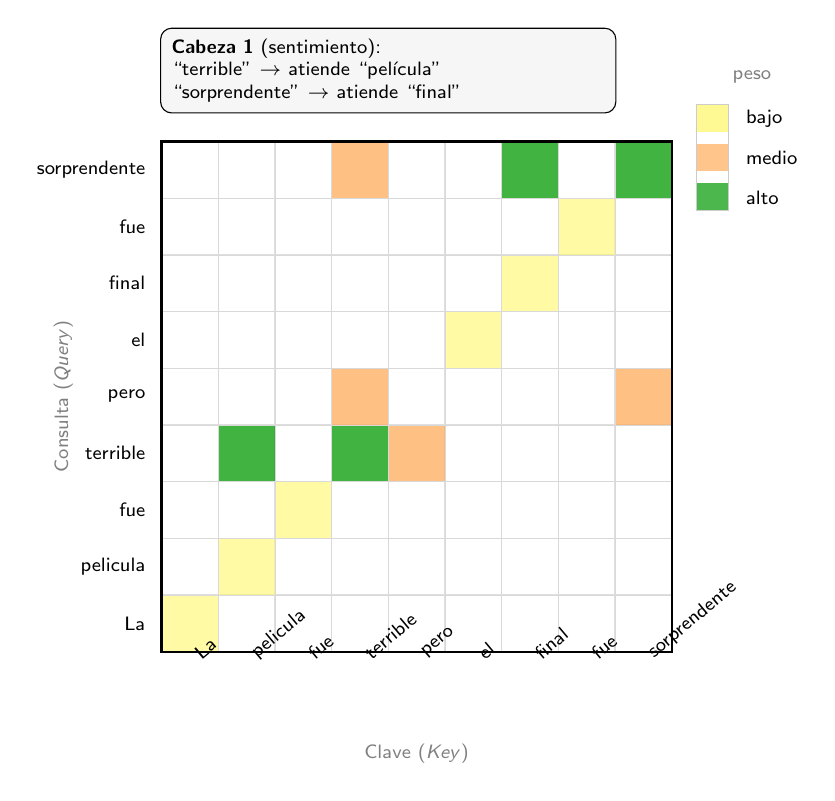
\begin{tikzpicture}[font=\sffamily\small]
\def\cs{0.72}
% Grilla base
\foreach \i in {0,...,8}{
  \foreach \j in {0,...,8}{
    \draw[gray!25, thin] (\j*\cs, \i*\cs) rectangle ++(\cs,\cs);
  }
}
% Pesos altos (verde)
\foreach \i/\j in {3/1, 3/3, 8/6, 8/8}{
  \fill[green!60!black, opacity=0.75] (\j*\cs, \i*\cs) rectangle ++(\cs,\cs);
}
% Pesos medios (naranja)
\foreach \i/\j in {3/4, 8/3, 4/3, 4/8}{
  \fill[orange!65, opacity=0.75] (\j*\cs, \i*\cs) rectangle ++(\cs,\cs);
}
% Pesos bajos / diagonal (amarillo)
\foreach \i/\j in {0/0, 1/1, 2/2, 5/5, 6/6, 7/7}{
  \fill[yellow!60, opacity=0.6] (\j*\cs, \i*\cs) rectangle ++(\cs,\cs);
}
% Redibujar bordes
\foreach \i in {0,...,8}{
  \foreach \j in {0,...,8}{
    \draw[gray!30, very thin] (\j*\cs, \i*\cs) rectangle ++(\cs,\cs);
  }
}
\draw[black, thick] (0,0) rectangle (9*\cs,9*\cs);
% Etiquetas eje X
\foreach \j/\w in {0/La,1/pelicula,2/fue,3/terrible,4/pero,
                   5/el,6/final,7/fue,8/sorprendente}{
  \node[font=\sffamily\scriptsize, rotate=40, anchor=west]
    at (\j*\cs+0.36,-0.12) {\w};
}
\node[font=\sffamily\scriptsize, text=gray, anchor=north]
  at (9*\cs/2,-1.05) {Clave (\textit{Key})};
% Etiquetas eje Y
\foreach \i/\w in {0/La,1/pelicula,2/fue,3/terrible,4/pero,
                   5/el,6/final,7/fue,8/sorprendente}{
  \node[font=\sffamily\scriptsize, anchor=east]
    at (-0.08,\i*\cs+0.36) {\w};
}
\node[font=\sffamily\scriptsize, text=gray, rotate=90, anchor=south]
  at (-1.0,9*\cs/2) {Consulta (\textit{Query})};
% Leyenda
\fill[yellow!60, opacity=0.7]      (6.8,6.60) rectangle ++(0.4,0.35);
\fill[orange!65, opacity=0.7]      (6.8,6.10) rectangle ++(0.4,0.35);
\fill[green!60!black, opacity=0.7] (6.8,5.60) rectangle ++(0.4,0.35);
\draw[gray!40] (6.8,5.60) rectangle ++(0.4,1.35);
\node[font=\sffamily\scriptsize, anchor=west] at (7.3,6.77) {bajo};
\node[font=\sffamily\scriptsize, anchor=west] at (7.3,6.27) {medio};
\node[font=\sffamily\scriptsize, anchor=west] at (7.3,5.77) {alto};
\node[font=\sffamily\scriptsize, text=gray]   at (7.5,7.3)  {peso};
% Anotación
\node[draw, rounded corners, fill=gray!7, inner sep=4pt,
      font=\sffamily\scriptsize, align=left, text width=5.5cm]
  at (4.0*\cs,9*\cs+0.9) {
    \textbf{Cabeza 1} (sentimiento):\\
    ``terrible'' $\to$ atiende ``pel\'icula''\\
    ``sorprendente'' $\to$ atiende ``final''
  };
\end{tikzpicture}
\caption*{D8 — Mapa de calor de pesos de atención}
\end{figure}

\newpage

% ----------------------------------------------------------------------------
% DIAGRAMA 9: Tabla de valores sinusoidales por posición
% Lámina: "Codificación Posicional"
% ----------------------------------------------------------------------------
\begin{figure}[h]\centering
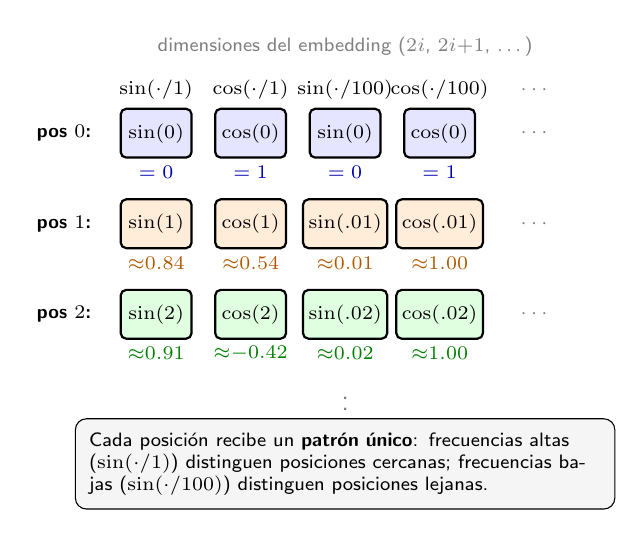
\begin{tikzpicture}[
  font=\sffamily\small,
  row/.style={draw, rounded corners=2pt, thick,
              minimum width=0.9cm, minimum height=0.62cm,
              inner sep=2pt, align=center},
  hdr/.style={font=\sffamily\scriptsize\bfseries, align=center},
  val/.style={font=\sffamily\scriptsize, align=center, text=blue!70!black}
]
\node[hdr] at (2.0,3.2) {$\sin(\cdot/1)$};
\node[hdr] at (3.2,3.2) {$\cos(\cdot/1)$};
\node[hdr] at (4.4,3.2) {$\sin(\cdot/100)$};
\node[hdr] at (5.6,3.2) {$\cos(\cdot/100)$};
\node[hdr, text=gray] at (6.8,3.2) {$\cdots$};
\node[font=\sffamily\scriptsize, text=gray] at (4.4,3.75)
  {dimensiones del embedding ($2i$, $2i{+}1$, \ldots)};
% pos 0
\node[font=\sffamily\scriptsize\bfseries, anchor=east] at (1.3,2.65) {pos $0$:};
\node[row, fill=blue!10] at (2.0,2.65) {\scriptsize$\sin(0)$};
\node[row, fill=blue!10] at (3.2,2.65) {\scriptsize$\cos(0)$};
\node[row, fill=blue!10] at (4.4,2.65) {\scriptsize$\sin(0)$};
\node[row, fill=blue!10] at (5.6,2.65) {\scriptsize$\cos(0)$};
\node[font=\sffamily\scriptsize, text=gray] at (6.8,2.65) {$\cdots$};
\node[val] at (2.0,2.15) {$= 0$};
\node[val] at (3.2,2.15) {$= 1$};
\node[val] at (4.4,2.15) {$= 0$};
\node[val] at (5.6,2.15) {$= 1$};
% pos 1
\node[font=\sffamily\scriptsize\bfseries, anchor=east] at (1.3,1.5) {pos $1$:};
\node[row, fill=orange!15] at (2.0,1.5) {\scriptsize$\sin(1)$};
\node[row, fill=orange!15] at (3.2,1.5) {\scriptsize$\cos(1)$};
\node[row, fill=orange!15] at (4.4,1.5) {\scriptsize$\sin(.01)$};
\node[row, fill=orange!15] at (5.6,1.5) {\scriptsize$\cos(.01)$};
\node[font=\sffamily\scriptsize, text=gray] at (6.8,1.5) {$\cdots$};
\node[val, text=orange!70!black] at (2.0,1.0) {${\approx}0.84$};
\node[val, text=orange!70!black] at (3.2,1.0) {${\approx}0.54$};
\node[val, text=orange!70!black] at (4.4,1.0) {${\approx}0.01$};
\node[val, text=orange!70!black] at (5.6,1.0) {${\approx}1.00$};
% pos 2
\node[font=\sffamily\scriptsize\bfseries, anchor=east] at (1.3,0.35) {pos $2$:};
\node[row, fill=green!12] at (2.0,0.35) {\scriptsize$\sin(2)$};
\node[row, fill=green!12] at (3.2,0.35) {\scriptsize$\cos(2)$};
\node[row, fill=green!12] at (4.4,0.35) {\scriptsize$\sin(.02)$};
\node[row, fill=green!12] at (5.6,0.35) {\scriptsize$\cos(.02)$};
\node[font=\sffamily\scriptsize, text=gray] at (6.8,0.35) {$\cdots$};
\node[val, text=green!50!black] at (2.0,-0.15) {${\approx}0.91$};
\node[val, text=green!50!black] at (3.2,-0.15) {${\approx}{-}0.42$};
\node[val, text=green!50!black] at (4.4,-0.15) {${\approx}0.02$};
\node[val, text=green!50!black] at (5.6,-0.15) {${\approx}1.00$};
\node[font=\sffamily, text=gray] at (4.4,-0.75) {$\vdots$};
\node[draw, rounded corners, fill=gray!8, inner sep=5pt,
      font=\sffamily\scriptsize, align=left, text width=6.5cm]
  at (4.4,-1.55)
  {Cada posici\'on recibe un \textbf{patr\'on \'unico}:
   frecuencias altas ($\sin(\cdot/1)$) distinguen posiciones cercanas;
   frecuencias bajas ($\sin(\cdot/100)$) distinguen posiciones lejanas.};
\end{tikzpicture}
\caption*{D9 — Tabla de codificación posicional}
\end{figure}

\newpage

% ----------------------------------------------------------------------------
% DIAGRAMA 10: Costo de entrenar BERT desde cero
% Lámina: "Vista Previa: Clase 5"
% ----------------------------------------------------------------------------
\begin{figure}[h]\centering
\begin{tikzpicture}[
  font=\sffamily\small,
  item/.style={draw, rounded corners=3pt, thick,
               minimum width=5.8cm, minimum height=0.72cm,
               inner sep=5pt, align=left},
  arr/.style={-{Stealth[length=2mm]}, thick, gray!60}
]
\node[draw, rounded corners=4pt, thick, fill=red!10,
      minimum width=6.0cm, minimum height=0.8cm,
      font=\sffamily\small\bfseries, align=center, text=red!70!black]
  (titulo) at (0,4.2) {Entrenar BERT desde cero requiere\ldots};
\node[item, fill=gray!10] (i1) at (0,3.1)
  {\textbf{Datos:}\quad m\'as de 100\,GB de texto};
\node[item, fill=gray!13] (i2) at (0,2.2)
  {\textbf{Hardware:}\quad 4\,--\,16 TPUs o GPUs};
\node[item, fill=gray!16] (i3) at (0,1.3)
  {\textbf{Tiempo:}\quad semanas de c\'omputo continuo};
\node[item, fill=gray!19] (i4) at (0,0.4)
  {\textbf{Presupuesto:}\quad millones de d\'olares};
\node[draw, rounded corners=4pt, thick, fill=blue!10,
      minimum width=6.0cm, minimum height=0.8cm,
      font=\sffamily\small, align=center]
  (concl) at (0,-0.65)
  {Soluci\'on: \textbf{fine-tuning} de modelos pre-entrenados};
\draw[arr] (titulo.south)--(i1.north);
\draw[arr] (i4.south)--(concl.north);
\end{tikzpicture}
\caption*{D10 — Costo de entrenar BERT}
\end{figure}

\end{document}
